\section{Two scale preconditioner}

Let us finally move on to the two-scale preconditioner. We showed in the previous part that using only the fine scale preconditioner was not a good idea when the number of quadrants increased (the number of iterations roughly doubles when the mesh size is divided by two). As explained in the theory chapter, the idea is to add a coarse part in the preconditioner (i.e. $M^{-1} = P^f + P^c$), consisting mainly of solving a problem with an interpolation degree $p=1$ with a geometric multigrid method, so that the number of iterations stays constant when we increase the number of quadrants.  

As in the previous section, the tests will be performed in two parts : first, we will analyze the performances of the two-scale preconditioner when there are no hanging nodes (but for both regular and distorted meshes) and then we will look at what happens when the forest of quadtrees is refined recursively and therefore the mesh is not conforming anymore. 

In the last subsection, we will also motivate the choice of using higher order degrees of interpolation. We will indeed look at the best degree to obtain a given accuracy in the solution, i.e. the degree for which we have the solution to a given problem on a given mesh in the shortest amount of time and that is accurate enough. 

\subsection{No hanging nodes}

Let us first present the problem we will solve in this part. We want our numerical solution to capture both low and high frequency modes so we will superpose a cosine with low frequency and a sine with a high frequency. As before, the domain is : $\Omega = \left[ -1;1 \right]^2$ and $\Gamma$ is the boundary. We will solve : 

\begin{align}
\nabla^2 u &= -\frac{\pi^2}{2}\cos(\frac{\pi}{2}x)\cos(\frac{\pi}{2}y) - 5\pi^2\sin(5\pi x)\sin(5\pi y) &\text{on $\Omega$} \label{eq:prob_two}\\
u &= 0  &\text{on $\Gamma$}
\end{align}

This problem has an analytic solution that is given by : 

$$ u(x,y) = \cos(\frac{\pi}{2}x)\cos(\frac{\pi}{2}y) + \frac{1}{10}\sin(5\pi x)\sin(5\pi y)$$

\begin{figure}
\centering
\includegraphics[scale=0.35]{Results/two_simple_sol.eps}
\caption{Numerical solution to problem \ref{eq:prob_two} using an interpolation of order $p=2$ and $1.0\:10^{6}$ degrees of freedom on a regular mesh with no hanging nodes. This numerical solution has been obtained by the PCG with the two scale preconditioner.}
\label{two_simple_sol}
\end{figure}


An example of a numerical solution obtained using the preconditioned conjugate gradients with the two scale preconditioner can be seen on figure \ref{two_simple_sol}. This solution has been obtained in only 8 iterations and with an interpolation of degree $p=2$. 

\subsubsection{Regular meshes}

Let us now look at what happens to the number of iterations when we decrease the mesh size for different degrees of interpolation. Table \ref{two_table_reg} shows the number of degrees of freedom for the different meshes used (indeed, for a given mesh, the higher the degree of the interpolation, the more global nodes we have). We can already see that, thanks to the coarse preconditioner, we are able to have a lot more degrees of freedom than in the case where we only had the fine preconditioner.

\begin{table}
\centering
\begin{tabular}{c|cccc}
\hline
Number of quadrants & $128^2$ & $256^2$ & $512^2$ & $1024^2$\\
\hline
$p=2$ & $6.6\:10^4$ & $2.6\:10^5$ & $1.1\:10^6$ & $4.2\:10^6$ \\
$p=4$ & $2.6\:10^5$ & $1.1\:10^6$ & $4.2\:10^6$ & $1.7\:10^7$ \\
$p=6$ & $5.9\:10^5$ & $2.4\:10^6$ & $9.4\:10^6$ & $3.8\:10^7$ \\
$p=8$ & $1.1\:10^6$ & $4.2\:10^6$ & $1.7\:10^7$ & $6.7\:10^7$ \\
\hline
\end{tabular}
\caption{Number of degrees of freedom for a regular mesh with different numbers of quadrants and for different degrees of interpolation.}
\label{two_table_reg}
\end{table}

\begin{figure}
\centering
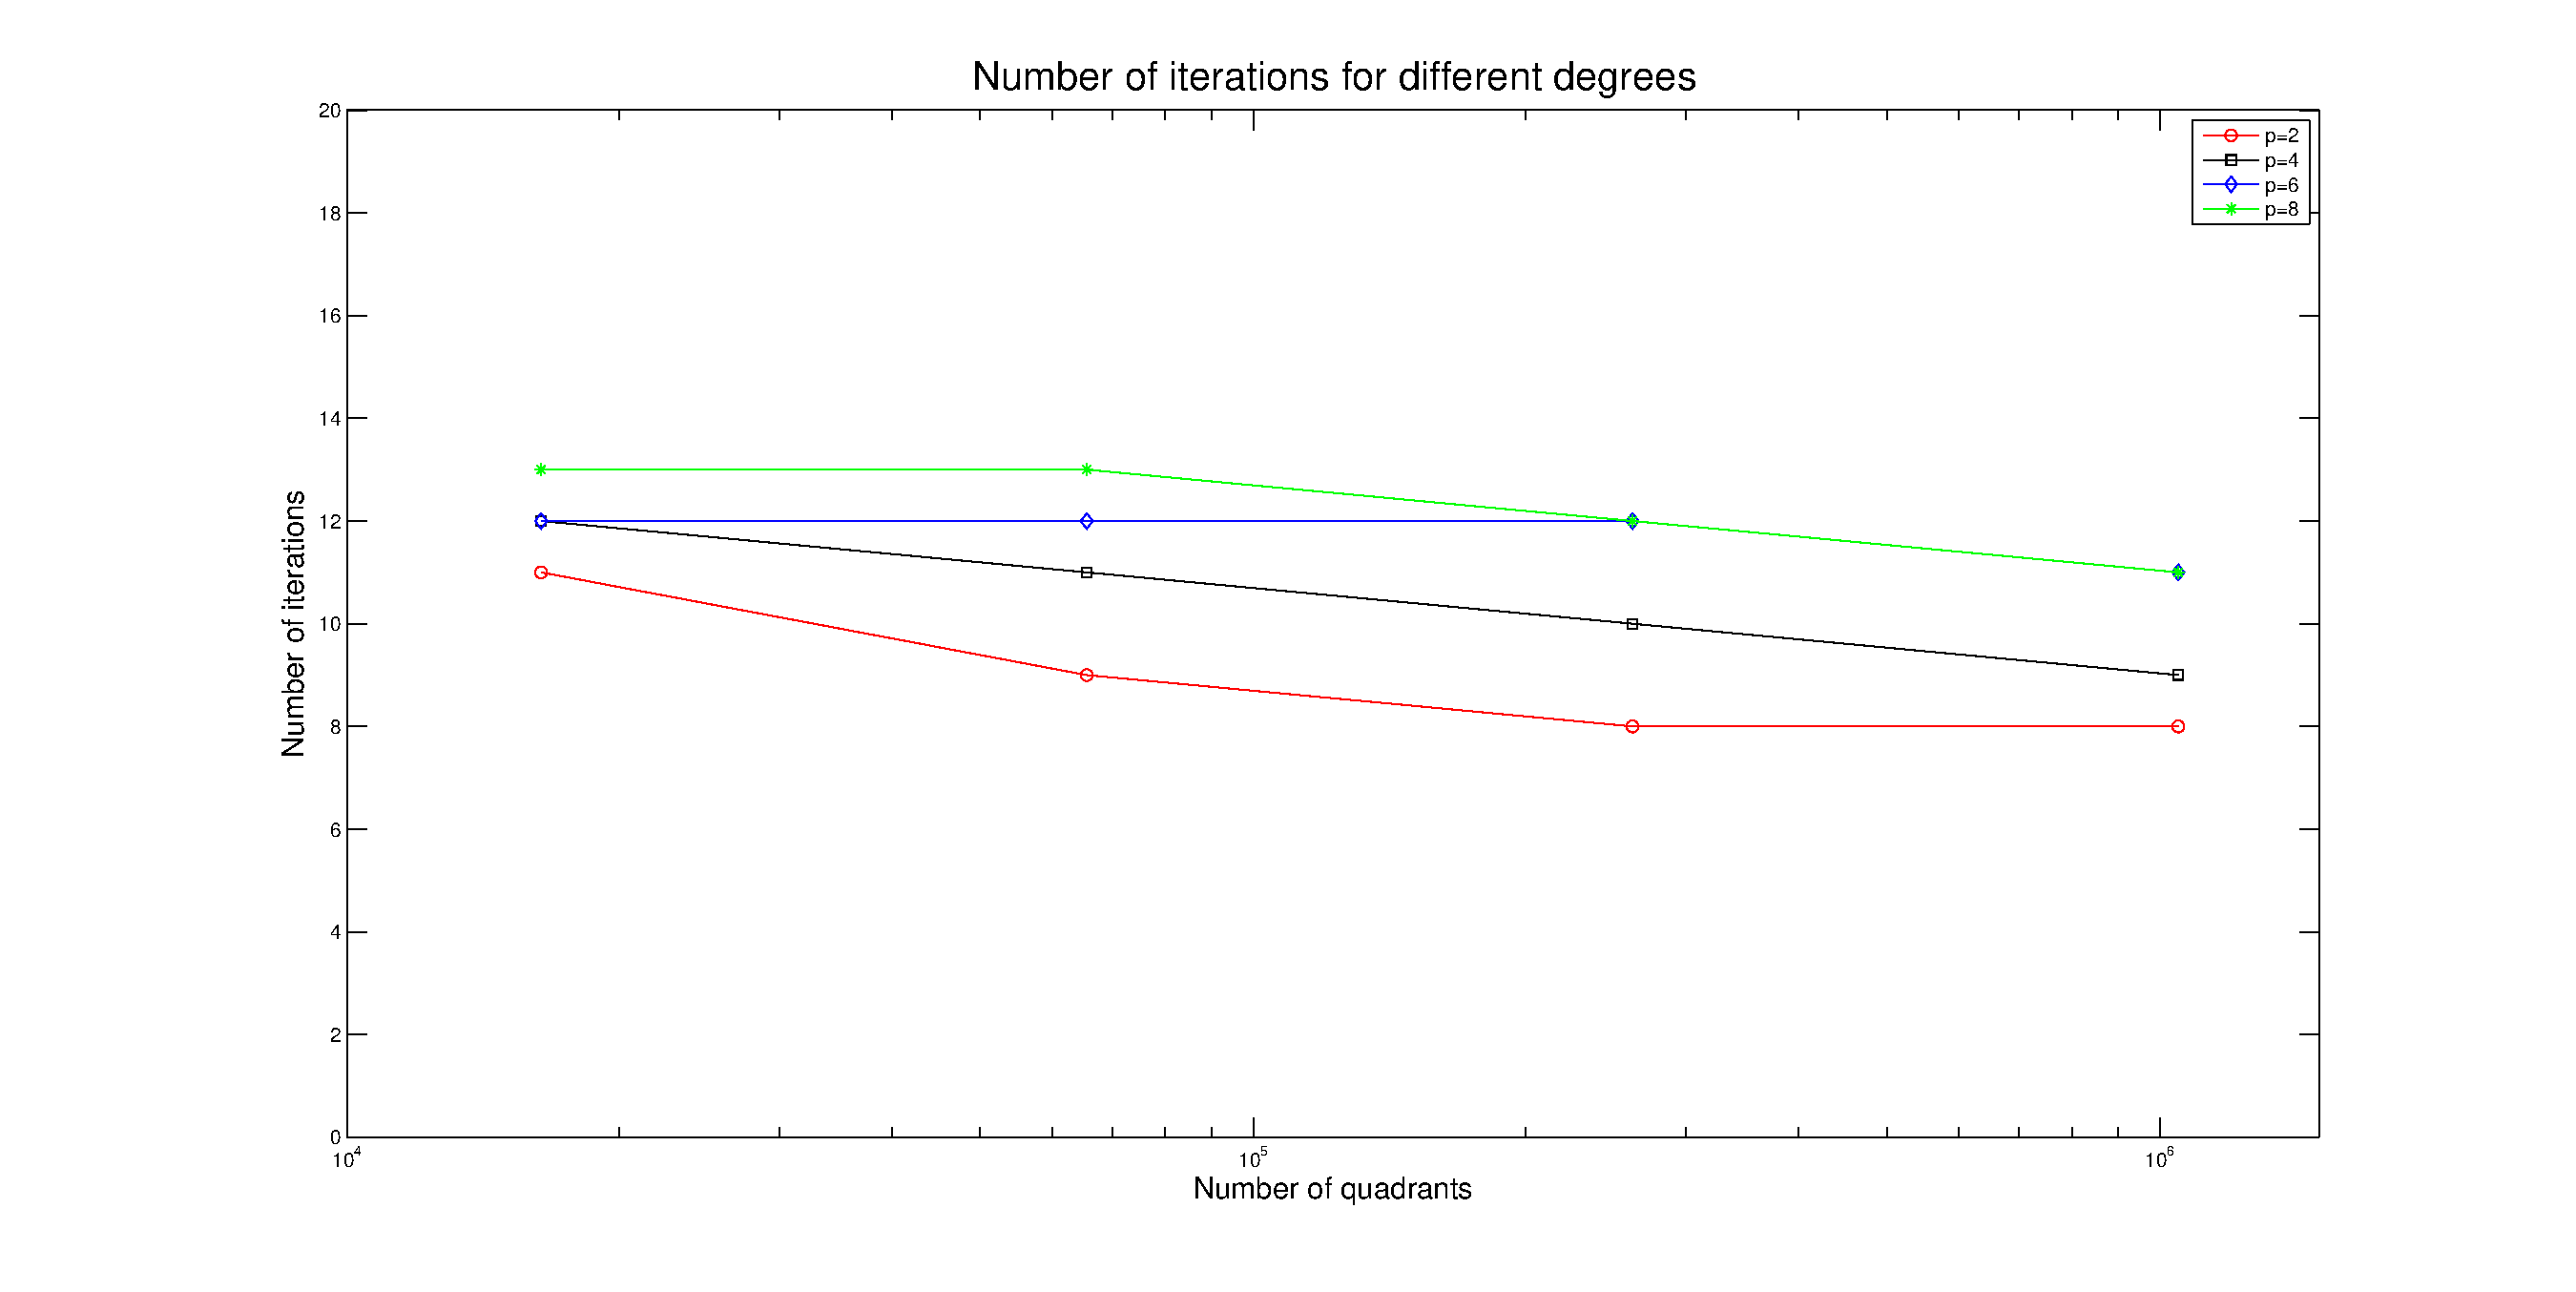
\includegraphics[scale=0.35]{Results/two_reg_iter.eps}
\caption{Number of iterations of PCG with the two scale preconditioner for degree $p$ of interpolation needed to reach the given tolerance of the norm of the residual as a function of the number of quadrants in a regular mesh.}
\label{two_reg_iter}
\end{figure}

For the following tests, we also have tighten the tolerance on the norm of the residual. We now require that : 

$$\frac{||r_k||_2}{||r_0||_2} < 10^{-5}$$

Figure \ref{two_reg_iter} shows the number of iterations needed to reach that tolerance of the norm of the residual when we use our two scale preconditioner for different degrees of interpolation. The first remark we can make is that the number of iterations does not increase with the number of quadrants (as it was the case when we only had the fine preconditioner). So we can conclude that the coarse preconditioner does the job it was designed to do. We can even note that the number of iterations slightly decreases. For example, for $p=6$, we need 12 iterations for $128^2$ quadrants but we only do 11 iterations for $1024^2$. An explanation for this phenomenon might be that when we increase the number of quadrants, we actually better separate the actions of the fine and coarse preconditioners and therefore the sum of the two is a better approximation of $A^{-1}$. We can mention that for $p=8$, we only need 11 iterations to solve a system that has more than 67 millions unknowns. 

A second remark we can make, as already observed when we only had the fine preconditioner, is that the number of iterations grows with the degree of the interpolation. For example, with $1024^2$ quadrants, we need 8 iterations when $p=2$ but we need to do 11 iterations when $p=8$. As before, this can be explained by the fact that as the degree of the interpolation increases, the size of the overlap decreases. A fixed sized overlap would fix this issue. 

\subsubsection{Meshes with distorted elements}

We will now look at what happens when the mesh is not regular but we have quadrants that are more and more distorted. We will use the same meshes already used in the previous section and obtained with the progression tool of GMSH (see figure \ref{fine_mesh_deform} for examples of such meshes).

\begin{figure}
\centering
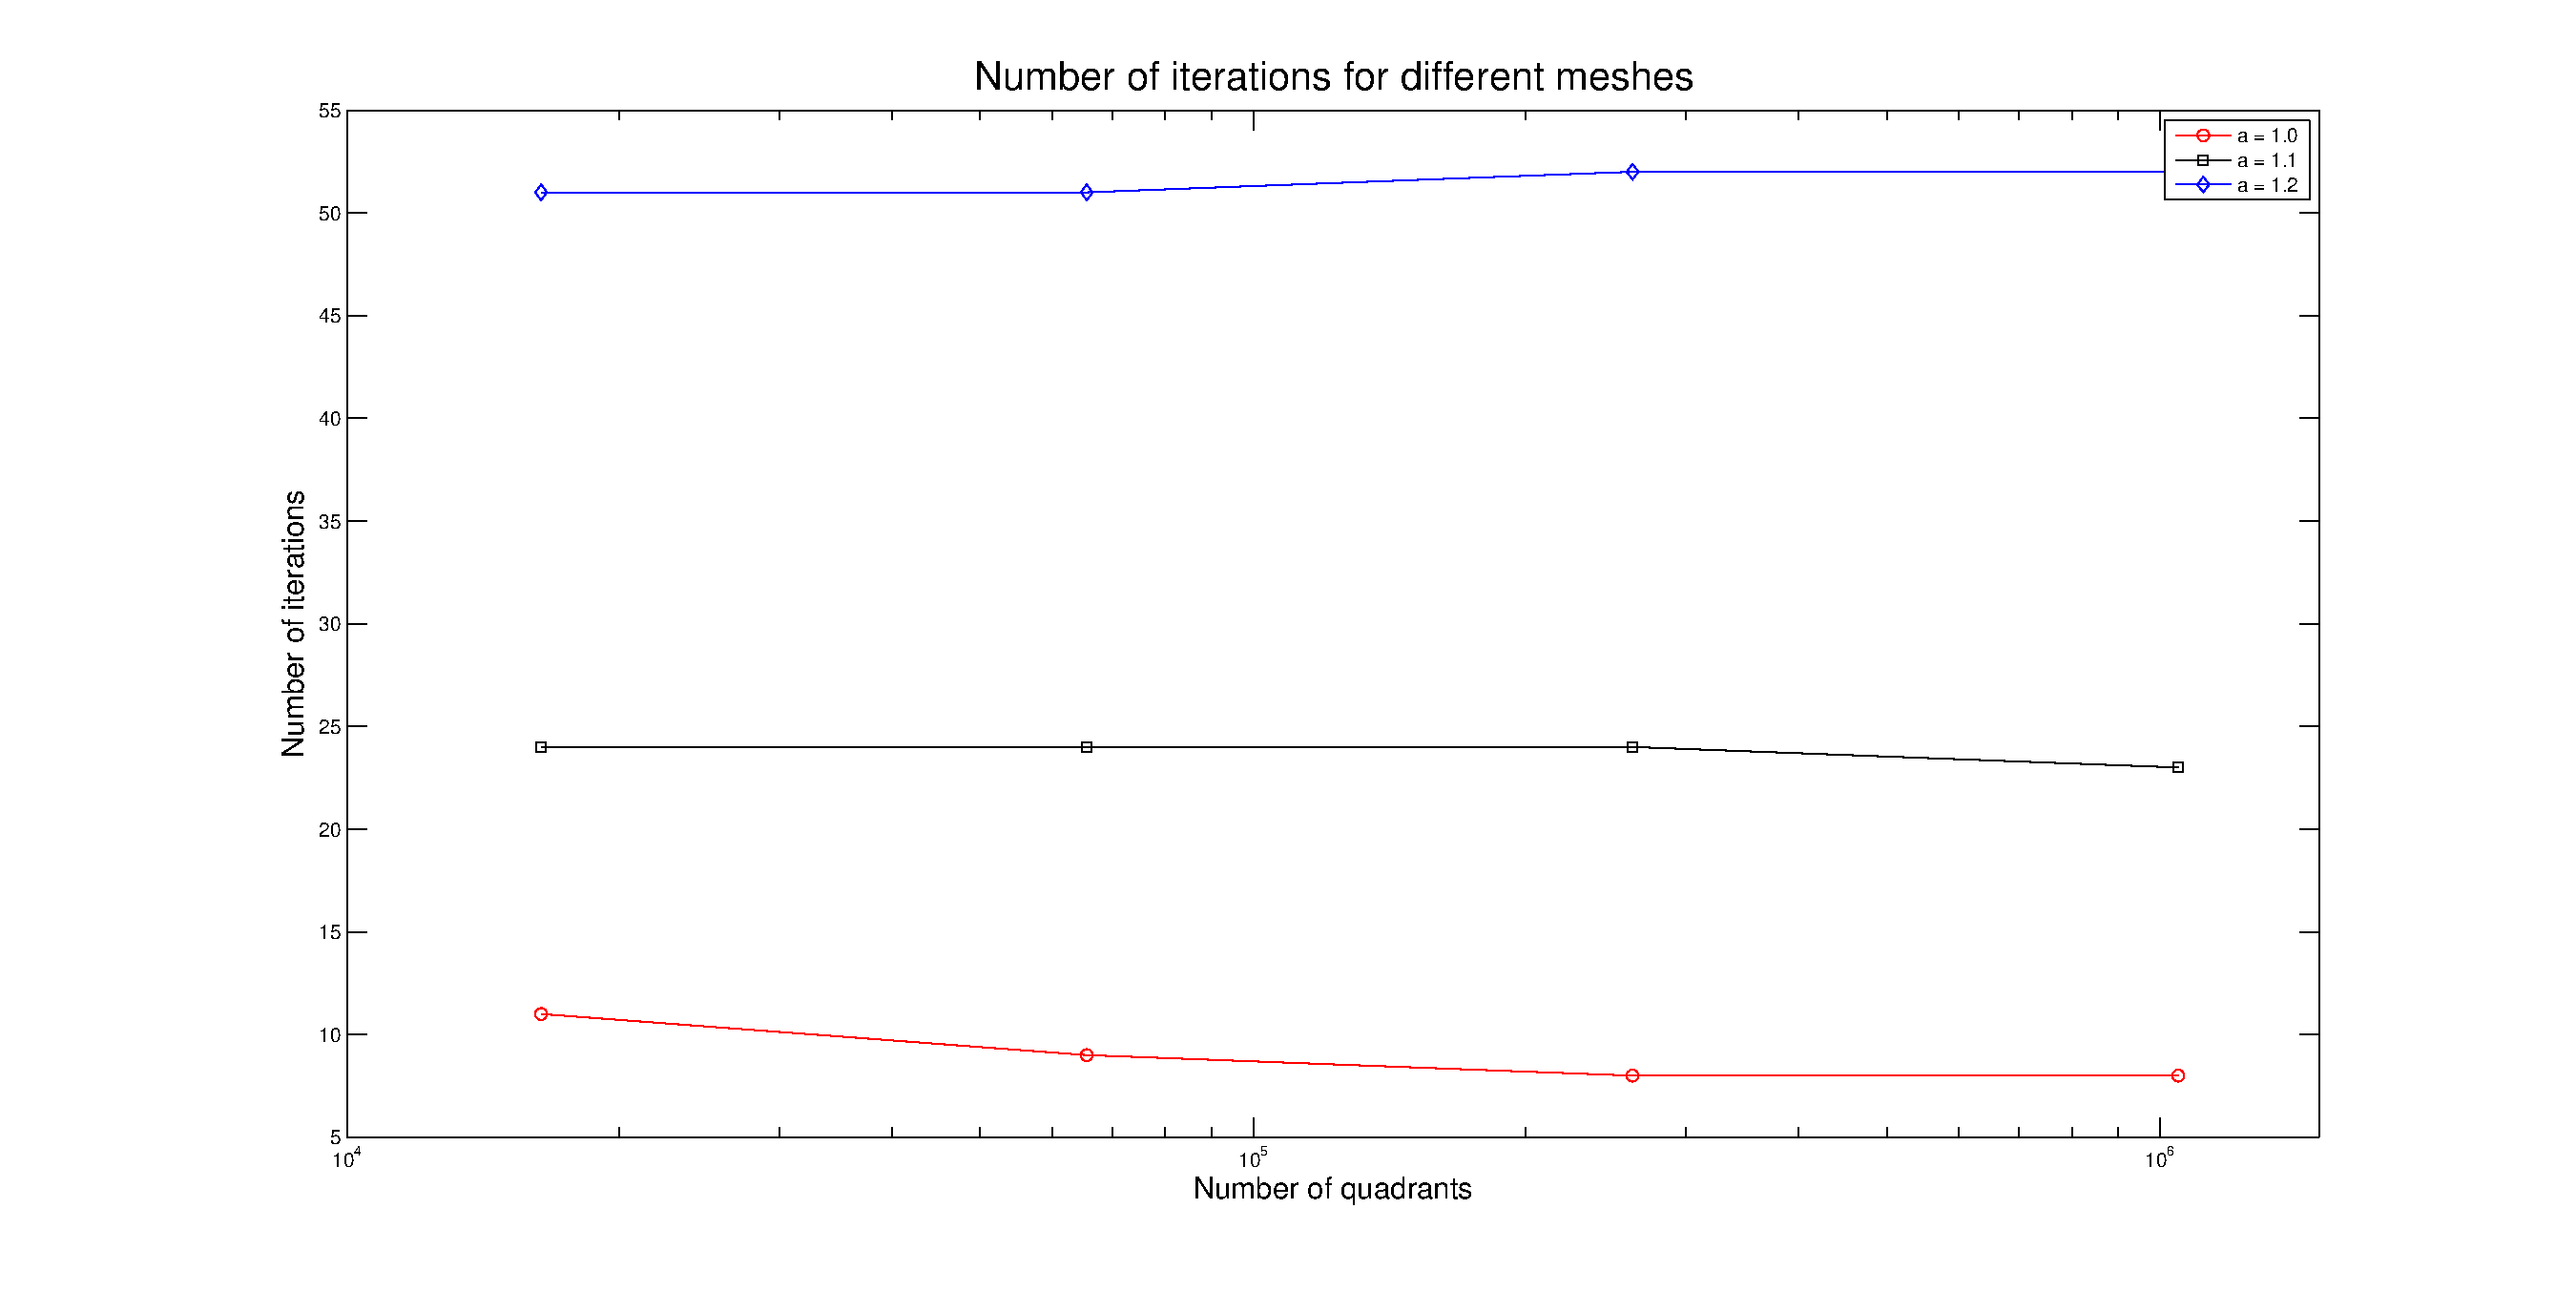
\includegraphics[scale=0.35]{Results/two_irreg_iter.eps}
\caption{Number of iterations of PCG with the two scale preconditioner for an interpolation degree $p=2$ needed to reach the given tolerance on the norm of the residual as a function of the number of quadrants for meshes with quadrants more and more distorted.}
\label{two_irreg_iter}
\end{figure}

For an interpolation of degree $p=2$, we looked at the number of iterations needed to reach the given tolerance as we increased the number of quadrants and for elements more and more distorted. Figure \ref{two_irreg_iter} shows the results. We can see that the number of iterations stays roughly the same when we increase the number of quadrants so once again the coarse part of the preconditioner does the job it is designed to do. 

We can also note that the more we distort the quadrants the more iterations we need to reach the given tolerance. This is to be expected since we developed the fine preconditioner to work optimally on quadrants aligned with the axis. This means that the more a quadrant is distorted the less accurate is the fine preconditioner part and therefore the more iterations we need. However, even with the most distorted mesh, the number of iterations stays acceptable and as explained in the previous section, the gain of not having to solve exactly on every quadrant is huge. We also have to say that the meshes presented here have an intrinsic structure since they are generated using the progression tool in GMSH. Therefore, the errors we make with our approximation are always in the same direction and the number of iterations needed increases. We might not have such an increase with a random mesh containing quadrants with the same quality measure. 


\subsection{Influence of hanging nodes}

Let us now move on to the cases where we have hanging nodes. As in the part with only the fine preconditioner, we will look at a problem where the solution has a jump so that we create hanging nodes when we use a recursive refine function in p4est. In addition to the hyperbolic tangent already presented in the previous subsection, we will include a high frequency sine wave to see how the grid adapts to capture it and how the two scale preconditioner performs in its presence. 

The problem we will solve is : 

\begin{align}
\nabla^2 u =& -2\tanh(12x)\tanh(12y)\left[ 12^2(1-\tanh(12x)^2) + 12^2(1-\tanh(12y)^2)\right] \nonumber \\
 &-  10\pi^2\sin(10\pi x)\sin(10\pi y) &\text{on $\Omega$} \label{eq:two_hang}\\
u =&   \tanh(12x)\tanh(12y) + \frac{1}{20}\sin(10\pi x)\sin(10\pi y)&\text{on $\Gamma$}
\end{align}

Where $\Omega = [-1;1]^2$ and $\Gamma$ is the boundary. This problem has an analytic solution that is given by : 

$$u(x,y) = \tanh(12x)\tanh(12y) + \frac{1}{20}\sin(10\pi x)\sin(10\pi y)$$

\begin{figure}
\centering
\includegraphics[scale=0.35]{Results/two_hang_plot.eps}
\caption{Numerical solution to problem \ref{eq:two_hang} using an interpolation of order $p=2$ on a non conforming mesh and obtained with PCG with the two scale preconditioner.}
\label{two_hang_plot}
\end{figure}

Figure \ref{two_hang_plot} shows an example of the numerical solution computed on a non conforming mesh with PCG and the two scale preconditioner. We can see on the plot both the steep jump due to the hyperbolic tangent and the small oscillations due to the sine wave.

\subsubsection{Increasing the relative number of hanging nodes}

Let us now look at the influence of increasing the number of hanging nodes in the mesh. To achieve this, we will use the same rule in the recursive refinement of the quadrants as in the previous section, given by relation \ref{hang_rel}. We will also tighten the parameter $tol$ used in order to have more quadrants than in the case when we only had the fine preconditioner. 

\begin{table}
\centering
\begin{tabular}{c|ccccccc}
Parameter $tol$ & 0.01 & 0.008 & 0.006 & 0.004 & 0.002 & 0.001 & 0.0005\\
\hline
Number of hanging nodes & 6080 & 8064 & 11008 & 14272 & 23200 & 33696 & 70112\\
Number of global nodes & 19921 & 25545 & 32265 & 49265 & 120201 & 208137 & 445425\\
$hang$ & 30.52\% & 31.57\% & 34.12\% & 28.97\% & 19.30\% & 16.19\% & 15.74\%
\end{tabular}
\caption{Statistics about the different meshes used for the tests regarding the influence of hanging nodes on the number of iterations as well as the ratio $hang$ defined by equation \ref{hang_frac}. The number of global and hanging nodes are for an interpolation degree $p=2$.}
\label{two_hang_table}
\end{table}

Table \ref{two_hang_table} shows some statistics about the different meshes used for the tests regarding the influence of hanging nodes on the number of iterations. The number of global and hanging nodes are for an interpolation of degree $p=2$ and the ratio $hang$ is given in equation \ref{hang_frac}.

We can see that, as expected, when we decrease the parameter $tol$, we have more hanging nodes. We can also see that, at first, tightening the parameter $tol$ increase the ratio $hang$ and we have more hanging nodes relatively to global nodes. Then, however, even though the number of hanging nodes still grows, the number of global nodes grows faster and therefore the ratio $hang$ decreases. This can be explained by the fact that if the parameter $tol$ is very low then we start to refine all part more equally (even the ones where the function does not vary a lot) and the relative number of hanging nodes drops. 

\begin{figure}
\centering
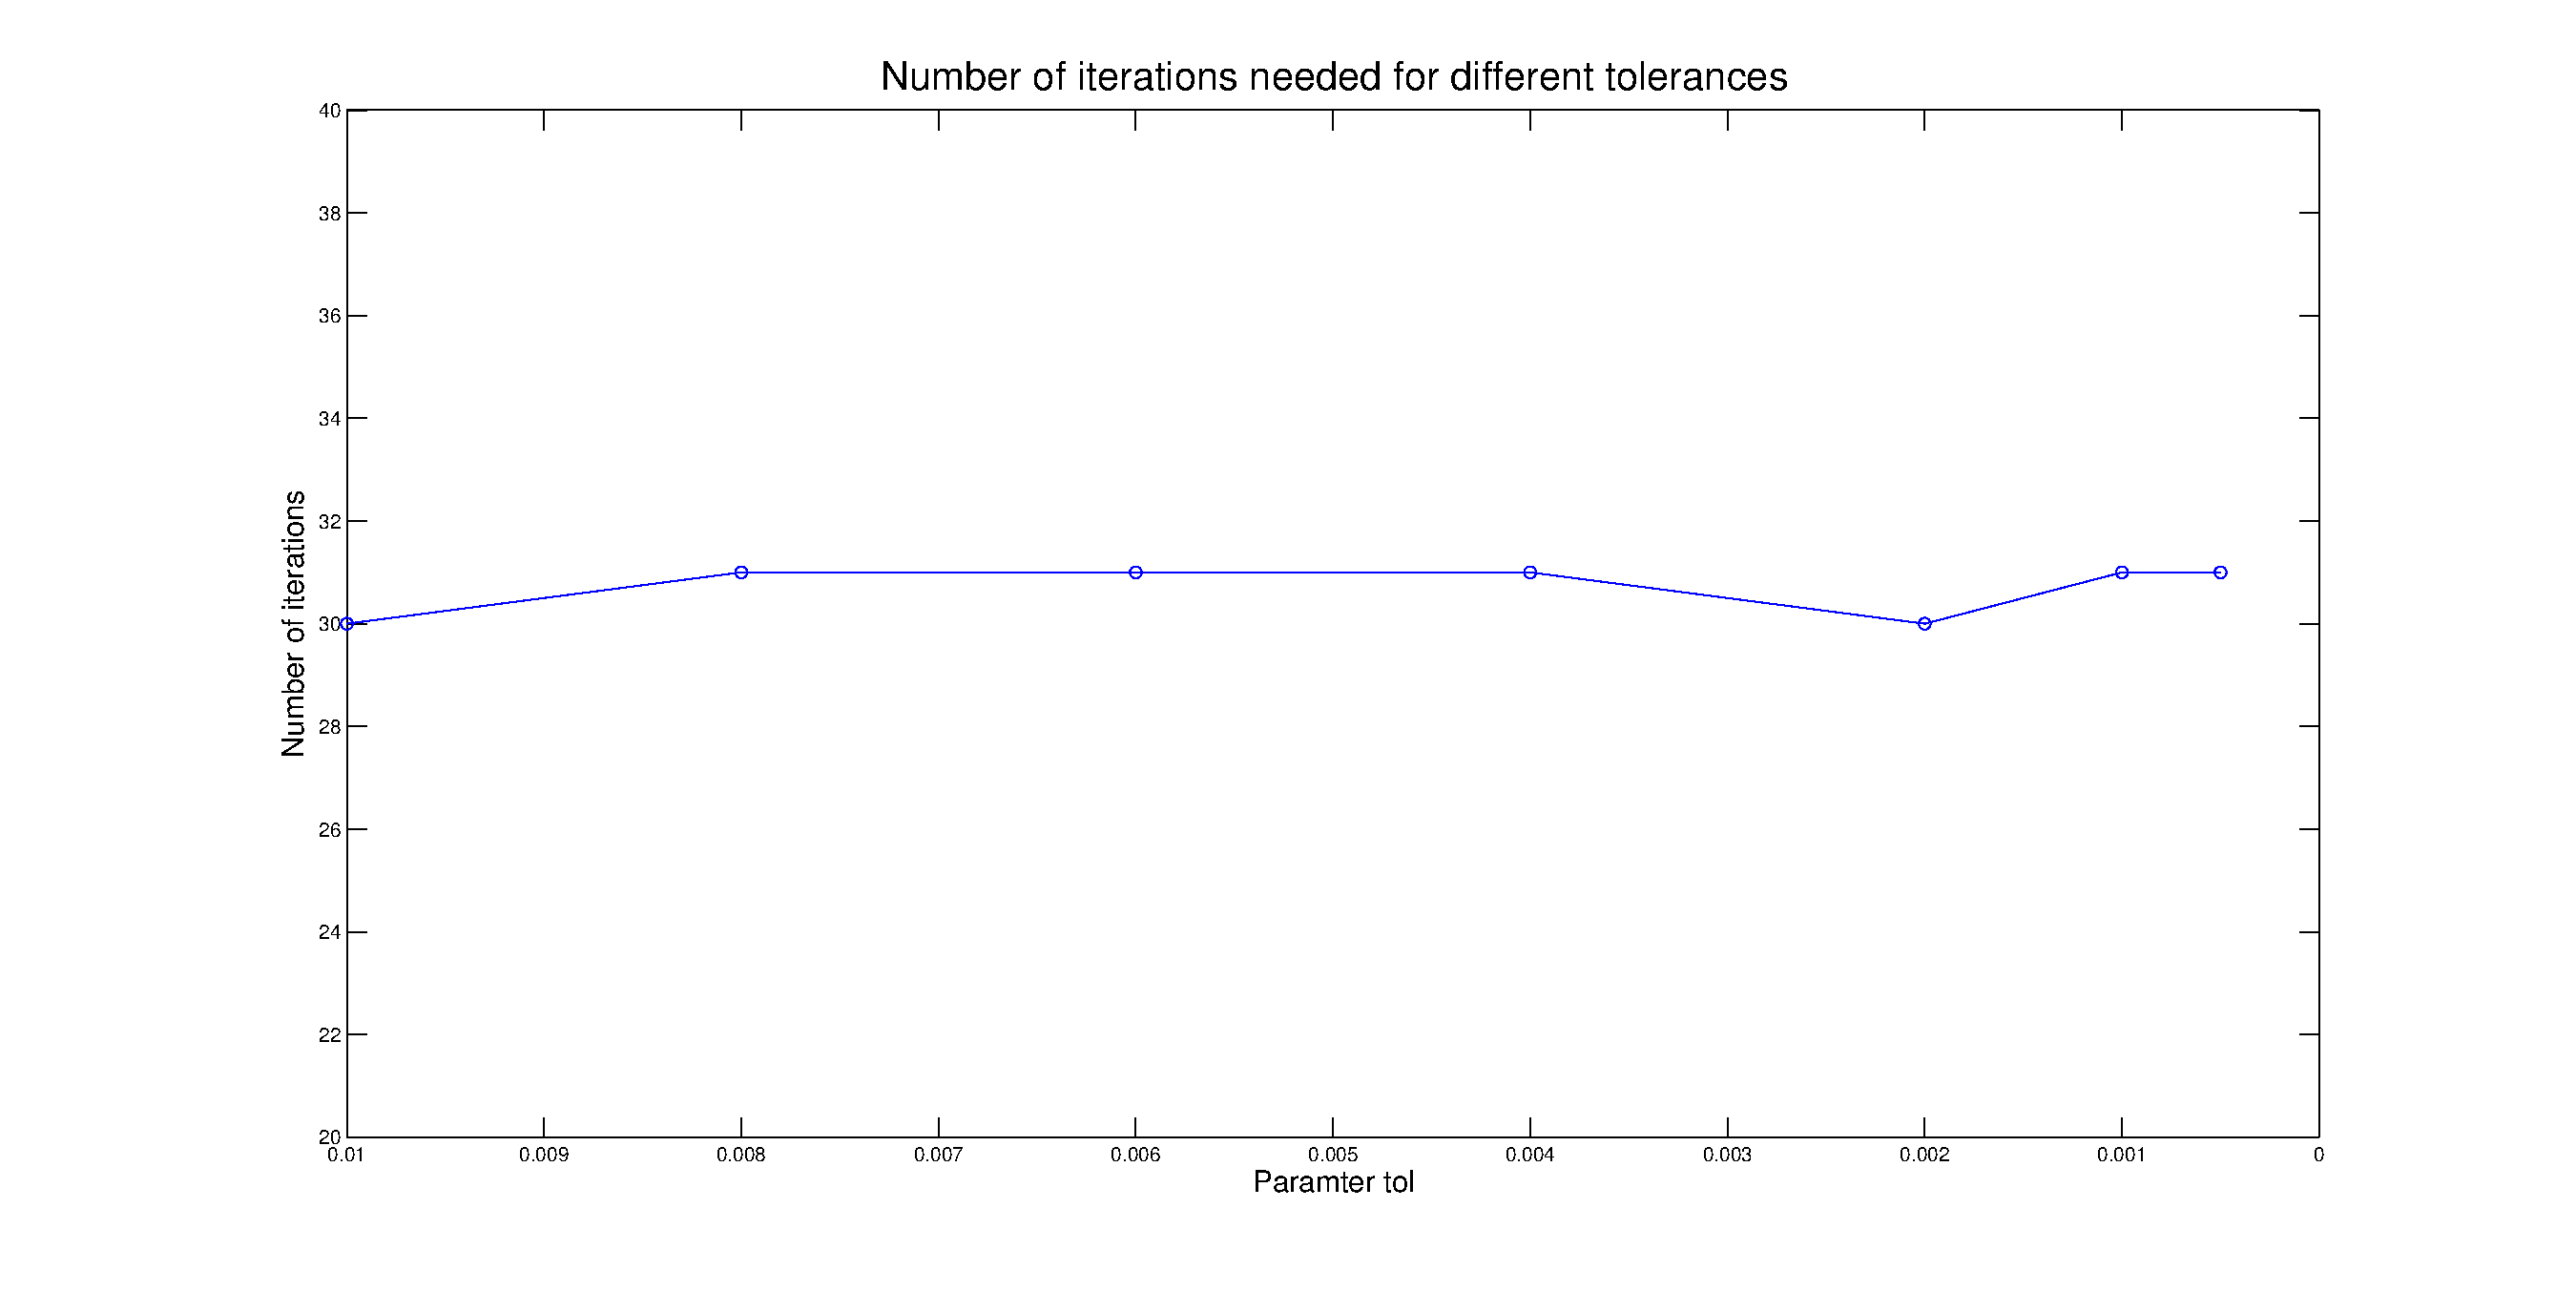
\includegraphics[scale=0.35]{Results/two_hang_iter.eps}
\caption{Number of iterations of PCG with the two scale preconditioner with a degree of interpolation $p=2$ on meshes with hanging nodes defined by the parameter $tol$.}
\label{two_hang_iter}
\end{figure}


Figure \ref{two_hang_iter} shows the number of iterations needed to reach the given tolerance with an interpolation degree $p=2$ on the different meshes presented in table \ref{two_hang_table}. We can see that the number of iterations stays roughly the same (it is either 30 or 31) for all meshes, whatever the number of hanging nodes and the value of the ratio $hang$. So we can conclude that the coarse preconditioner once again guaranties the h-independent convergence and that the number of hanging nodes does not have a great influence on the number of iterations. 

We also have to note that, for the same problem, if we use a conforming mesh, the number of iterations needed drops to 16. So even if the number of hanging nodes (absolute or relative) does not greatly influence the number of iterations, just adding one non conforming quadrant does a lot to decrease the performance of the preconditioner. We can point the fact that, as mentioned earlier, when we have hanging quadrants, we do not handle every possibilities to compute the residuals in the overlaps. We can thus see how that affects the number of iterations. 


\subsubsection{Increasing the degree of the interpolation}

\begin{figure}
\centering
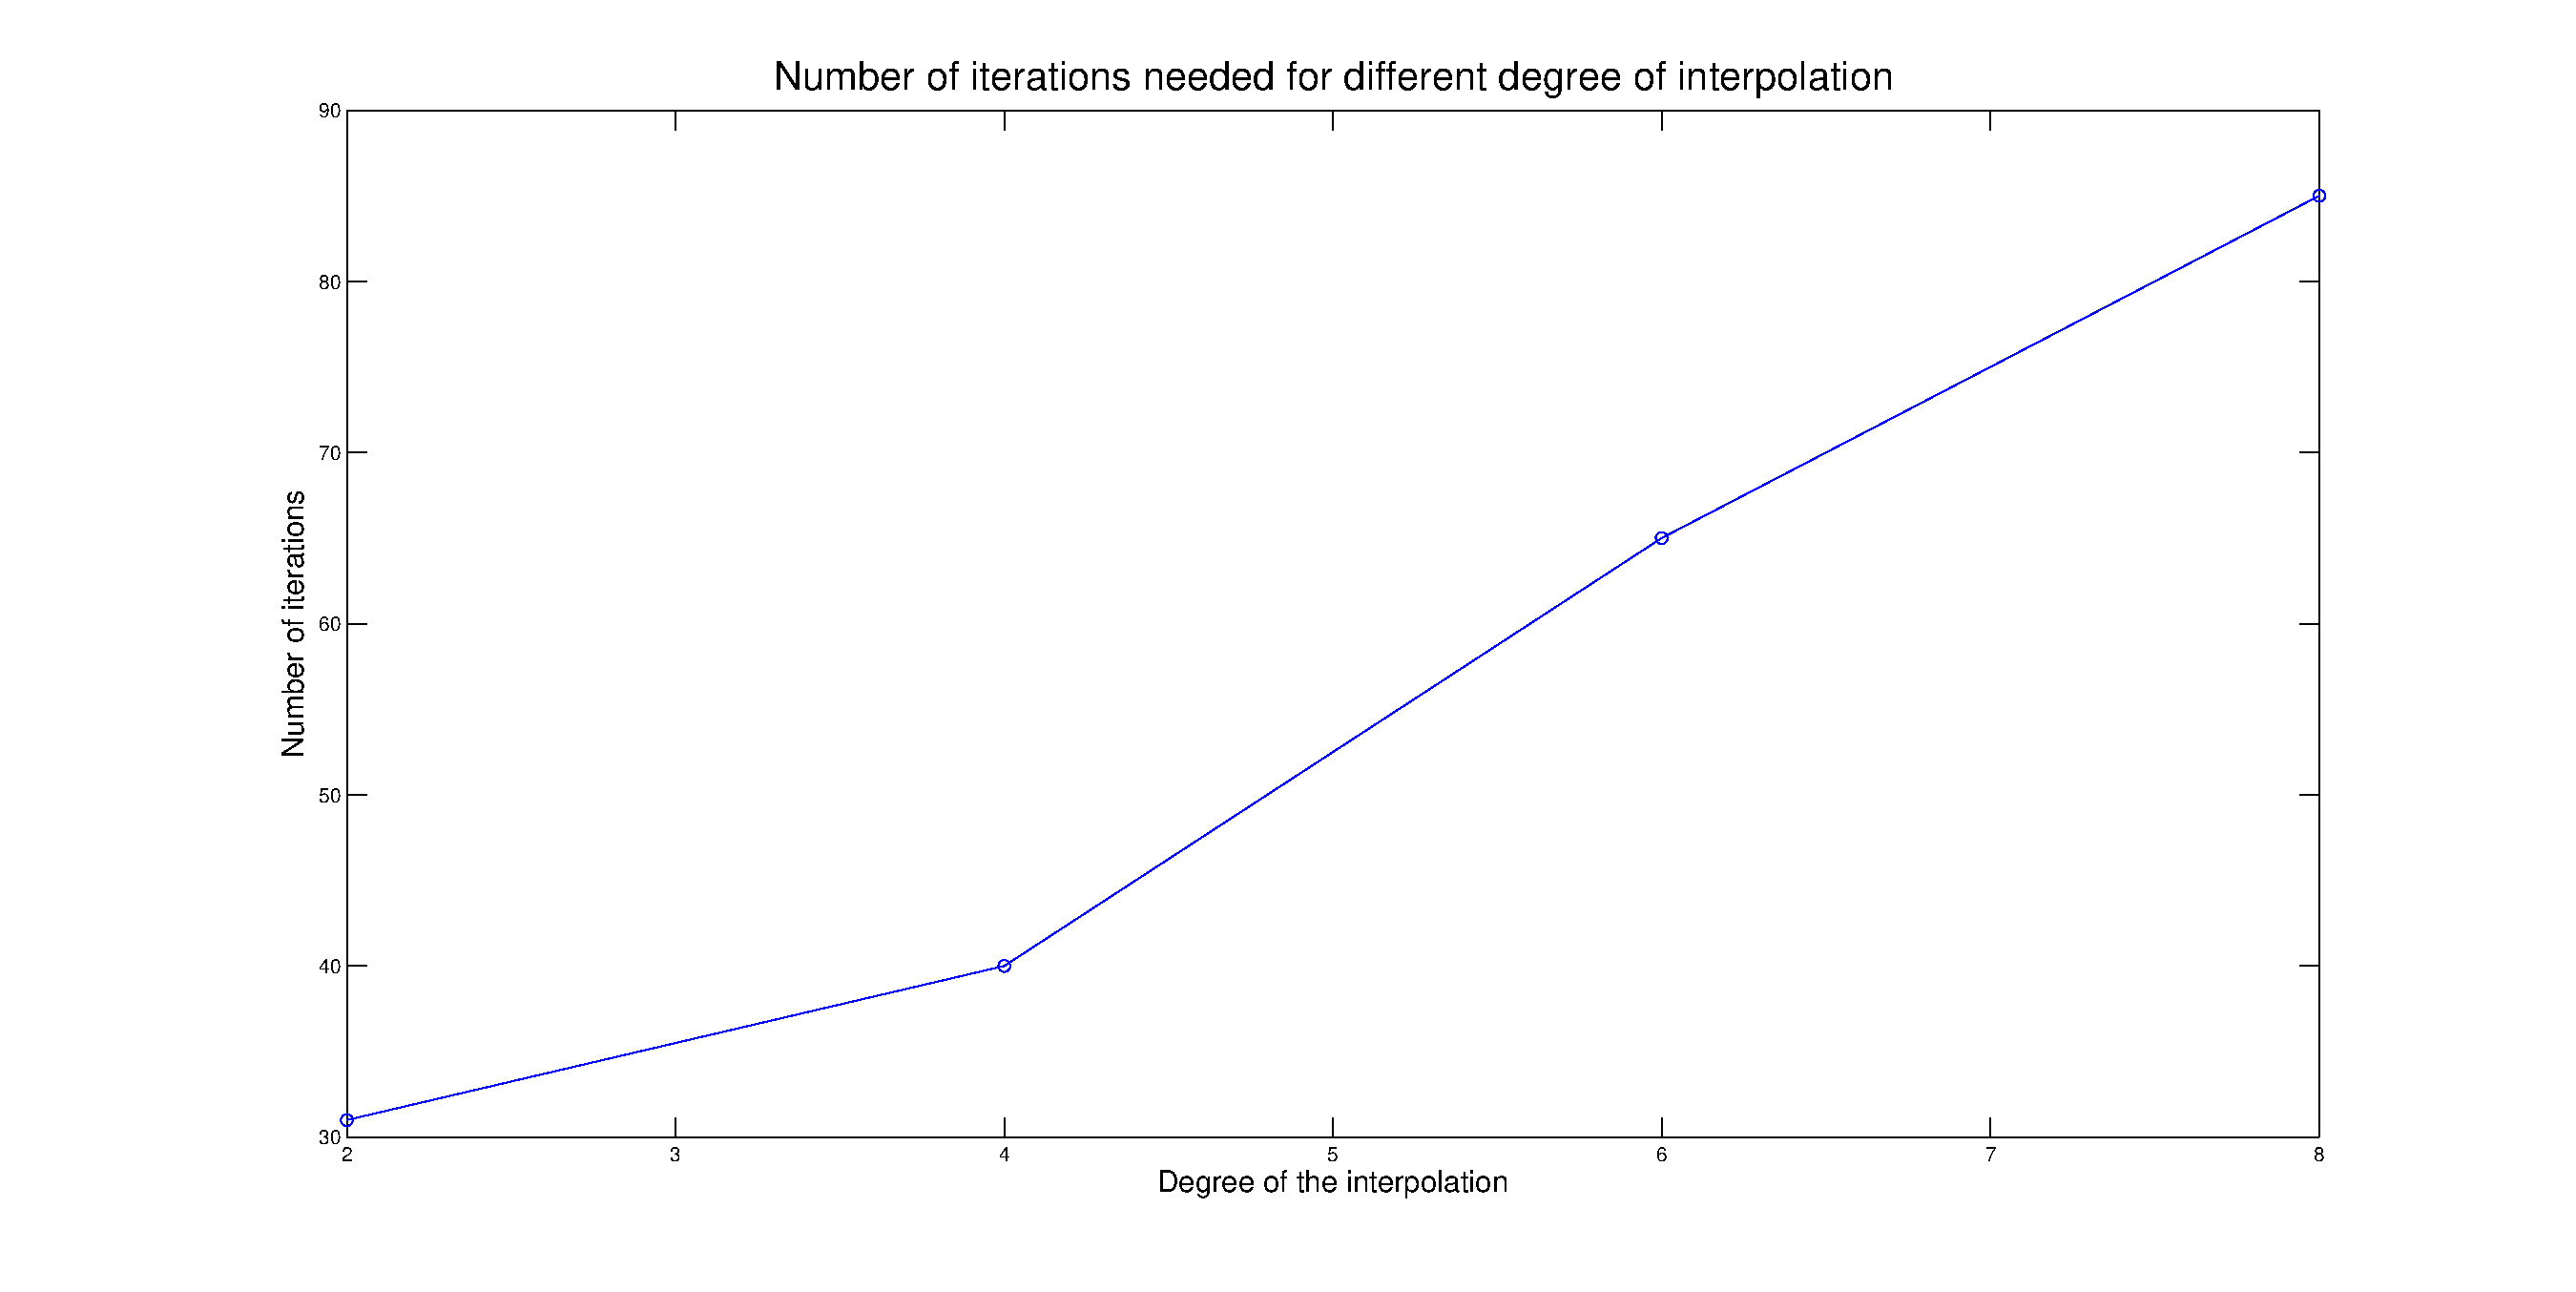
\includegraphics[scale=0.35]{Results/two_hang_deg.eps}
\caption{Number of iterations of PCG with the two scale preconditioner as a function of the degree of the interpolation used for a mesh obtained with $tol = 0.001$ in the recursive refine function.}
\label{two_hang_deg}
\end{figure}

Let us now move on to look at what happens when we increase the degree of the interpolation. We will use the mesh defined by $tol = 0.001$ and look at the number of iterations needed to reach the given tolerance for $p=2,4,6,8$. Figure \ref{two_hang_deg} shows the results. 

We can see that as we increase the degree of the interpolation, the number of iterations increases. It goes from 31 for $p=2$ to 85 iterations when $p=8$. We can see that it is quite a lot. But we also have to note that going from degree 2 to degree 8, we have also gone from $2.1\:10^5$ degrees of freedom to $3.4\:10^6$.

As in the case when we only had the fine preconditioner, several factors can be put forward to explain the increase in the number of iterations. First, when we increase the degree, the size of the overlap decreases and therefore the fine preconditioner is less effective. As mentioned in \cite{overlap_constant}, a fixed sized overlap would fix the issue. 

Second, we can say that the number of hanging nodes in the overlaps increases with the degree of the interpolation. Since we do not treat all possibilities when handling hanging quadrants, the error made is more important when we have a lot of nodes in the overlaps.


\subsection{Most efficient degree to obtain a given accuracy}

In this subsection, we will look at the best degree of interpolation $p$ to obtain a given accuracy. We will use the problem defined by \ref{eq:prob_two} and the distorted mesh using the progression tool of GMSH with $a=1.2$ that we will uniformly refine. We will also tighten the tolerance on the norm of the residual since we want the error to come from the interpolation and not from the fact that we only solve the linear system approximately. We will impose that : 

$$ \frac{||r_k||_2}{||r_0||_2} < 10^{-12} $$

Afterwards, we will compute the error committed by the discretization in the $L^2$-norm. Let us define $e^p$, the error made by using an interpolation of degree $p$, $u^p$ the solution of the discretized problem using a degree $p$, $U^p_i$ the numerical solution at the global node $i$ of the linear system that arises and $m_i$ the mass matrix associated with the integration. Then we have :  

\begin{align}
e^p &= \left( \int_\Omega (u-u^p)^2dxdy \right)^\frac{1}{2}\\
 &\approx \left( \sum_i (u(x_i,y_i)-U_i^p)^2 m_i \right)^\frac{1}{2}
\end{align}

We can note that if we refine uniformly the mesh, then $e^p$ will decrease but it will also cost us more. And for a given mesh, we have that $e^p$ decreases as $p$ increases (but it also costs us to increase the degree). So the question that arises is when is it more interesting to refine the mesh uniformly and when is it better to increase the degree of the interpolation to get the accuracy we want.

We will select degree $p$ to be the best for an accuracy of $10^{-a}$ if and only if there is a mesh such that $e^p<10^{-a}$ on this mesh and the time needed to obtain the numerical solution is smaller than for any degree on any other mesh and the same accuracy. 

\begin{figure}
\centering
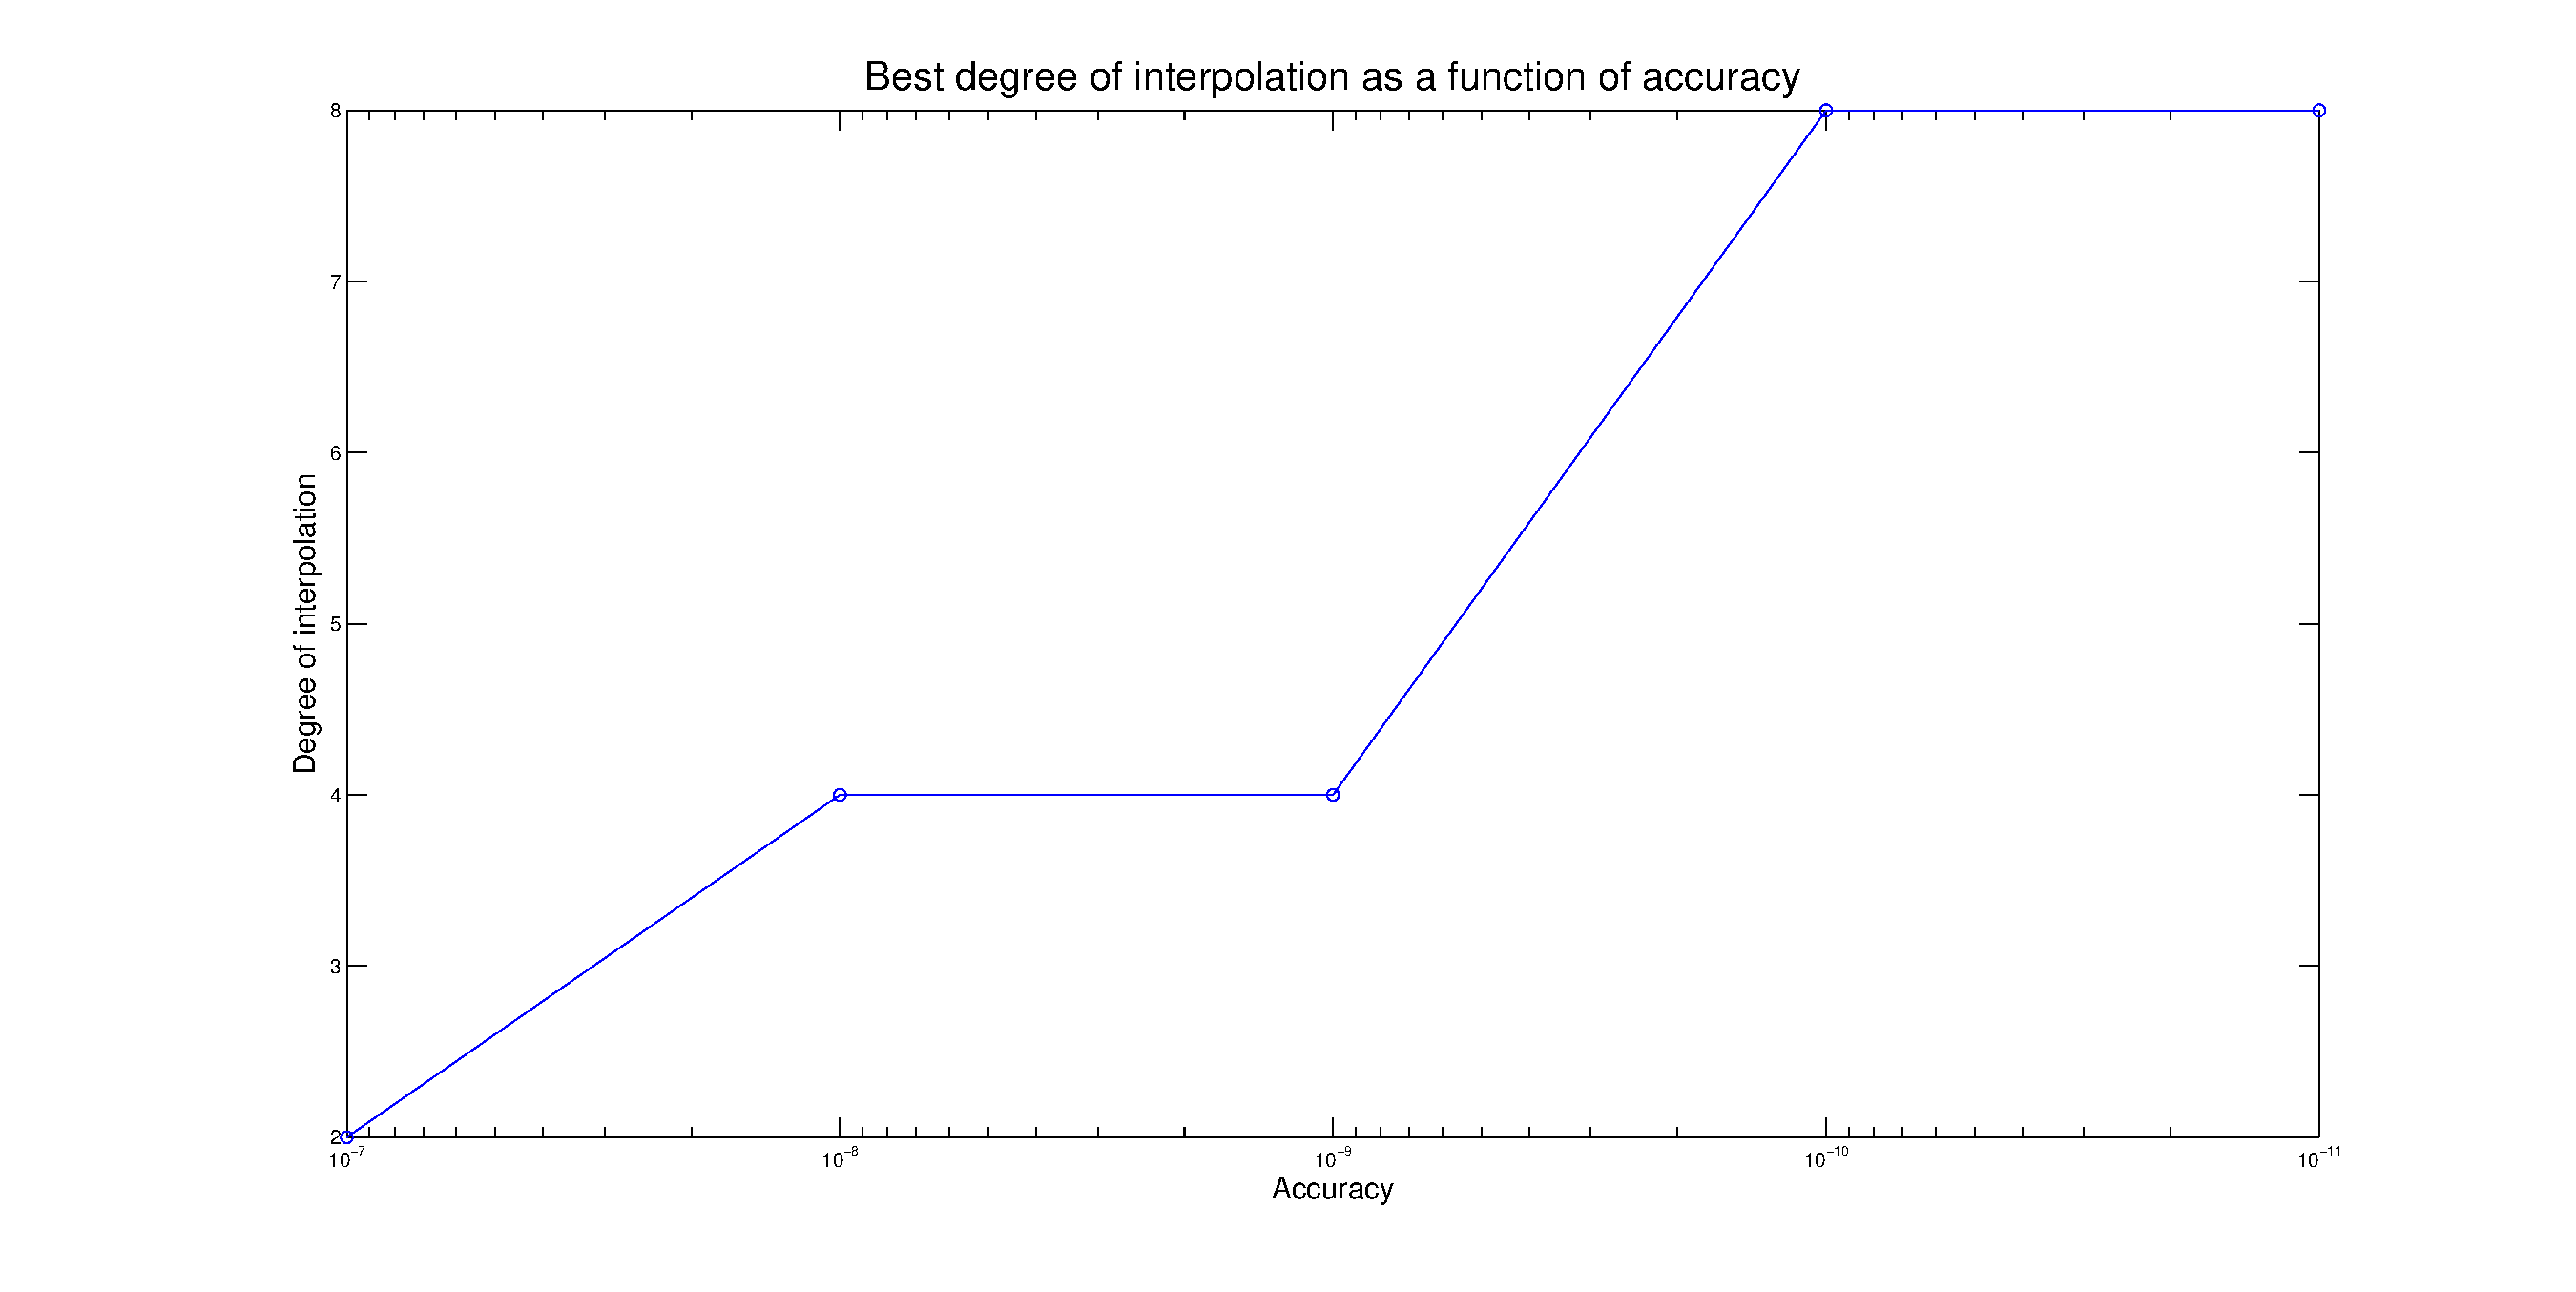
\includegraphics[scale=0.35]{Results/two_acc.eps}
\caption{Best degree of interpolation to solve problem \ref{eq:prob_two} on a distorted mesh as a function of the accuracy we want on the $L^2$-norm.}
\label{two_acc}
\end{figure}

Figure \ref{two_acc} shows the results. We can see that when the wanted accuracy is rather low (for $10^{-7}$) then it is quicker to use an order of interpolation $p=2$ because the number of iterations needed to solve the linear system is smaller than for a higher order interpolation. Moreover, the number of degrees of freedom to obtain such an accuracy is not so high as to make one iteration very long. 

On the other hand, when we want a better accuracy ($10^{-10}$, $10^{-11}$) then it is cheaper to use higher order interpolation such as $p=8$. This can be explained by the fact that, even though the number of iterations of PCG is higher (as mentioned earlier in this section), the number of degrees of freedom to obtain the wanted accuracy is much lower for $p=8$ than for the other degrees. Therefore, one iteration takes much less time and $p=8$ becomes more efficient. 

In between the two ($10^{-8}$, $10^{-9}$), we can see that the best degree is $p=4$ where we have a trade-off between the number of iterations needed to solve the system and the number of degrees of freedom.

The quantitative results presented here depend of course of the implementation, the problem to solve and the mesh used. However, we can note that the qualitative result stays true : the more accurate we want to be, the more interesting it becomes to use higher degree in the interpolation because then the number of DOF does not grow as large as it would with lower order polynomials. 




